\chapter{Real-Life Measurements}

\section{Introduction}

idkmybffjill

\section{Needle Probe Measurement Fundamentals}

Needle probe measurements were taken using an apparatus borrowed from the Cold
Regions Research and Engineering Laboratory, illustrated in figure
\ref{fig:apparatus}. Encased in a Pelican case for protection are a Campbell
CR10X data logger, a relay switch, a 12v gel cell for the CR10X and a series of
D-cells to power the heating coils in the needle. The program that came with the
data logger uses the relay switch to control the heat flux from the needle, and
records temperature data from the needle's thermocouple, as well as the voltage
across the heating element, over the course of a five minute heating curve and
a ten minute cooling curve.

\begin{figure}[h]
\centering
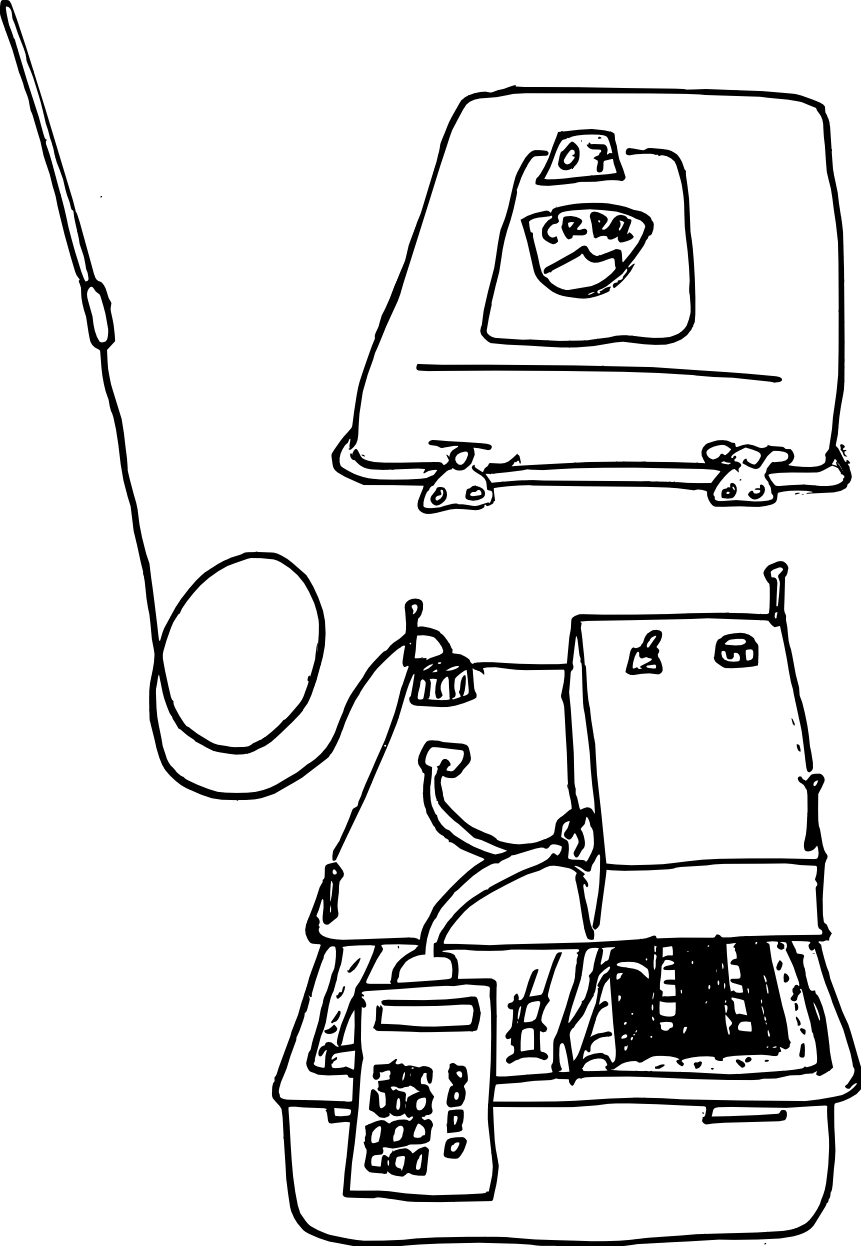
\includegraphics[width=0.7\textwidth]{fig/apparatus.png}
\label{fig:apparatus}
\caption{Extruded illustration of the needle probe apparatus. Major parts are labelled.}
\end{figure}

The apparatus is controlled using a keypad that enables one to communicate
with the data logger using Campbell ``star-codes.'' Initiating a test is a
matter of clearing and setting some registers using these star-codes.

\marginpar{source star codes?}

In general, the apparatus is used like so:

\begin{enumerate}
\item Turn on device.
\item Insert needle into medium being measured.
\item Use star-codes to clear the first three registers. ``* 6 A'' accesses the
registers, and ``D \(n\)'' toggles the \(n\)th register. For example, to clear
the second register, press ``* 6 A D 2'' .
\item Turn on the first register by pressing ``* 6 A D 1''. This makes the
apparatus measure temperature.
\item Turn on the second register by pressing ``* 6 A D 2''. This turns on the
heating element, effectively starting the test.
\item Wait 15 minutes for test to complete.
\end{enumerate}

Once testing is complete, data may be uploaded from the data logger using
Campbell's PC200X software and a particular series of cables and devices, as
shown in figure \ref{fig:cable}. In order, from datalogger to computer, they
are:

\marginpar{Source PC200X?}

\begin{enumerate}
\item A DE-9 cable
\item an SC32A optically isolating RS-232 interface
\item A DB-25-to-DE-9 serial cable
\item A DE-9 Null Modem cable
\item (Optional) A DE-9-to-USB cable
\end{enumerate}

Given the correct cables and ports, one may be able to decrease the number of
cables to two, plus the SC32A interface.

\begin{figure}[h]
\centering
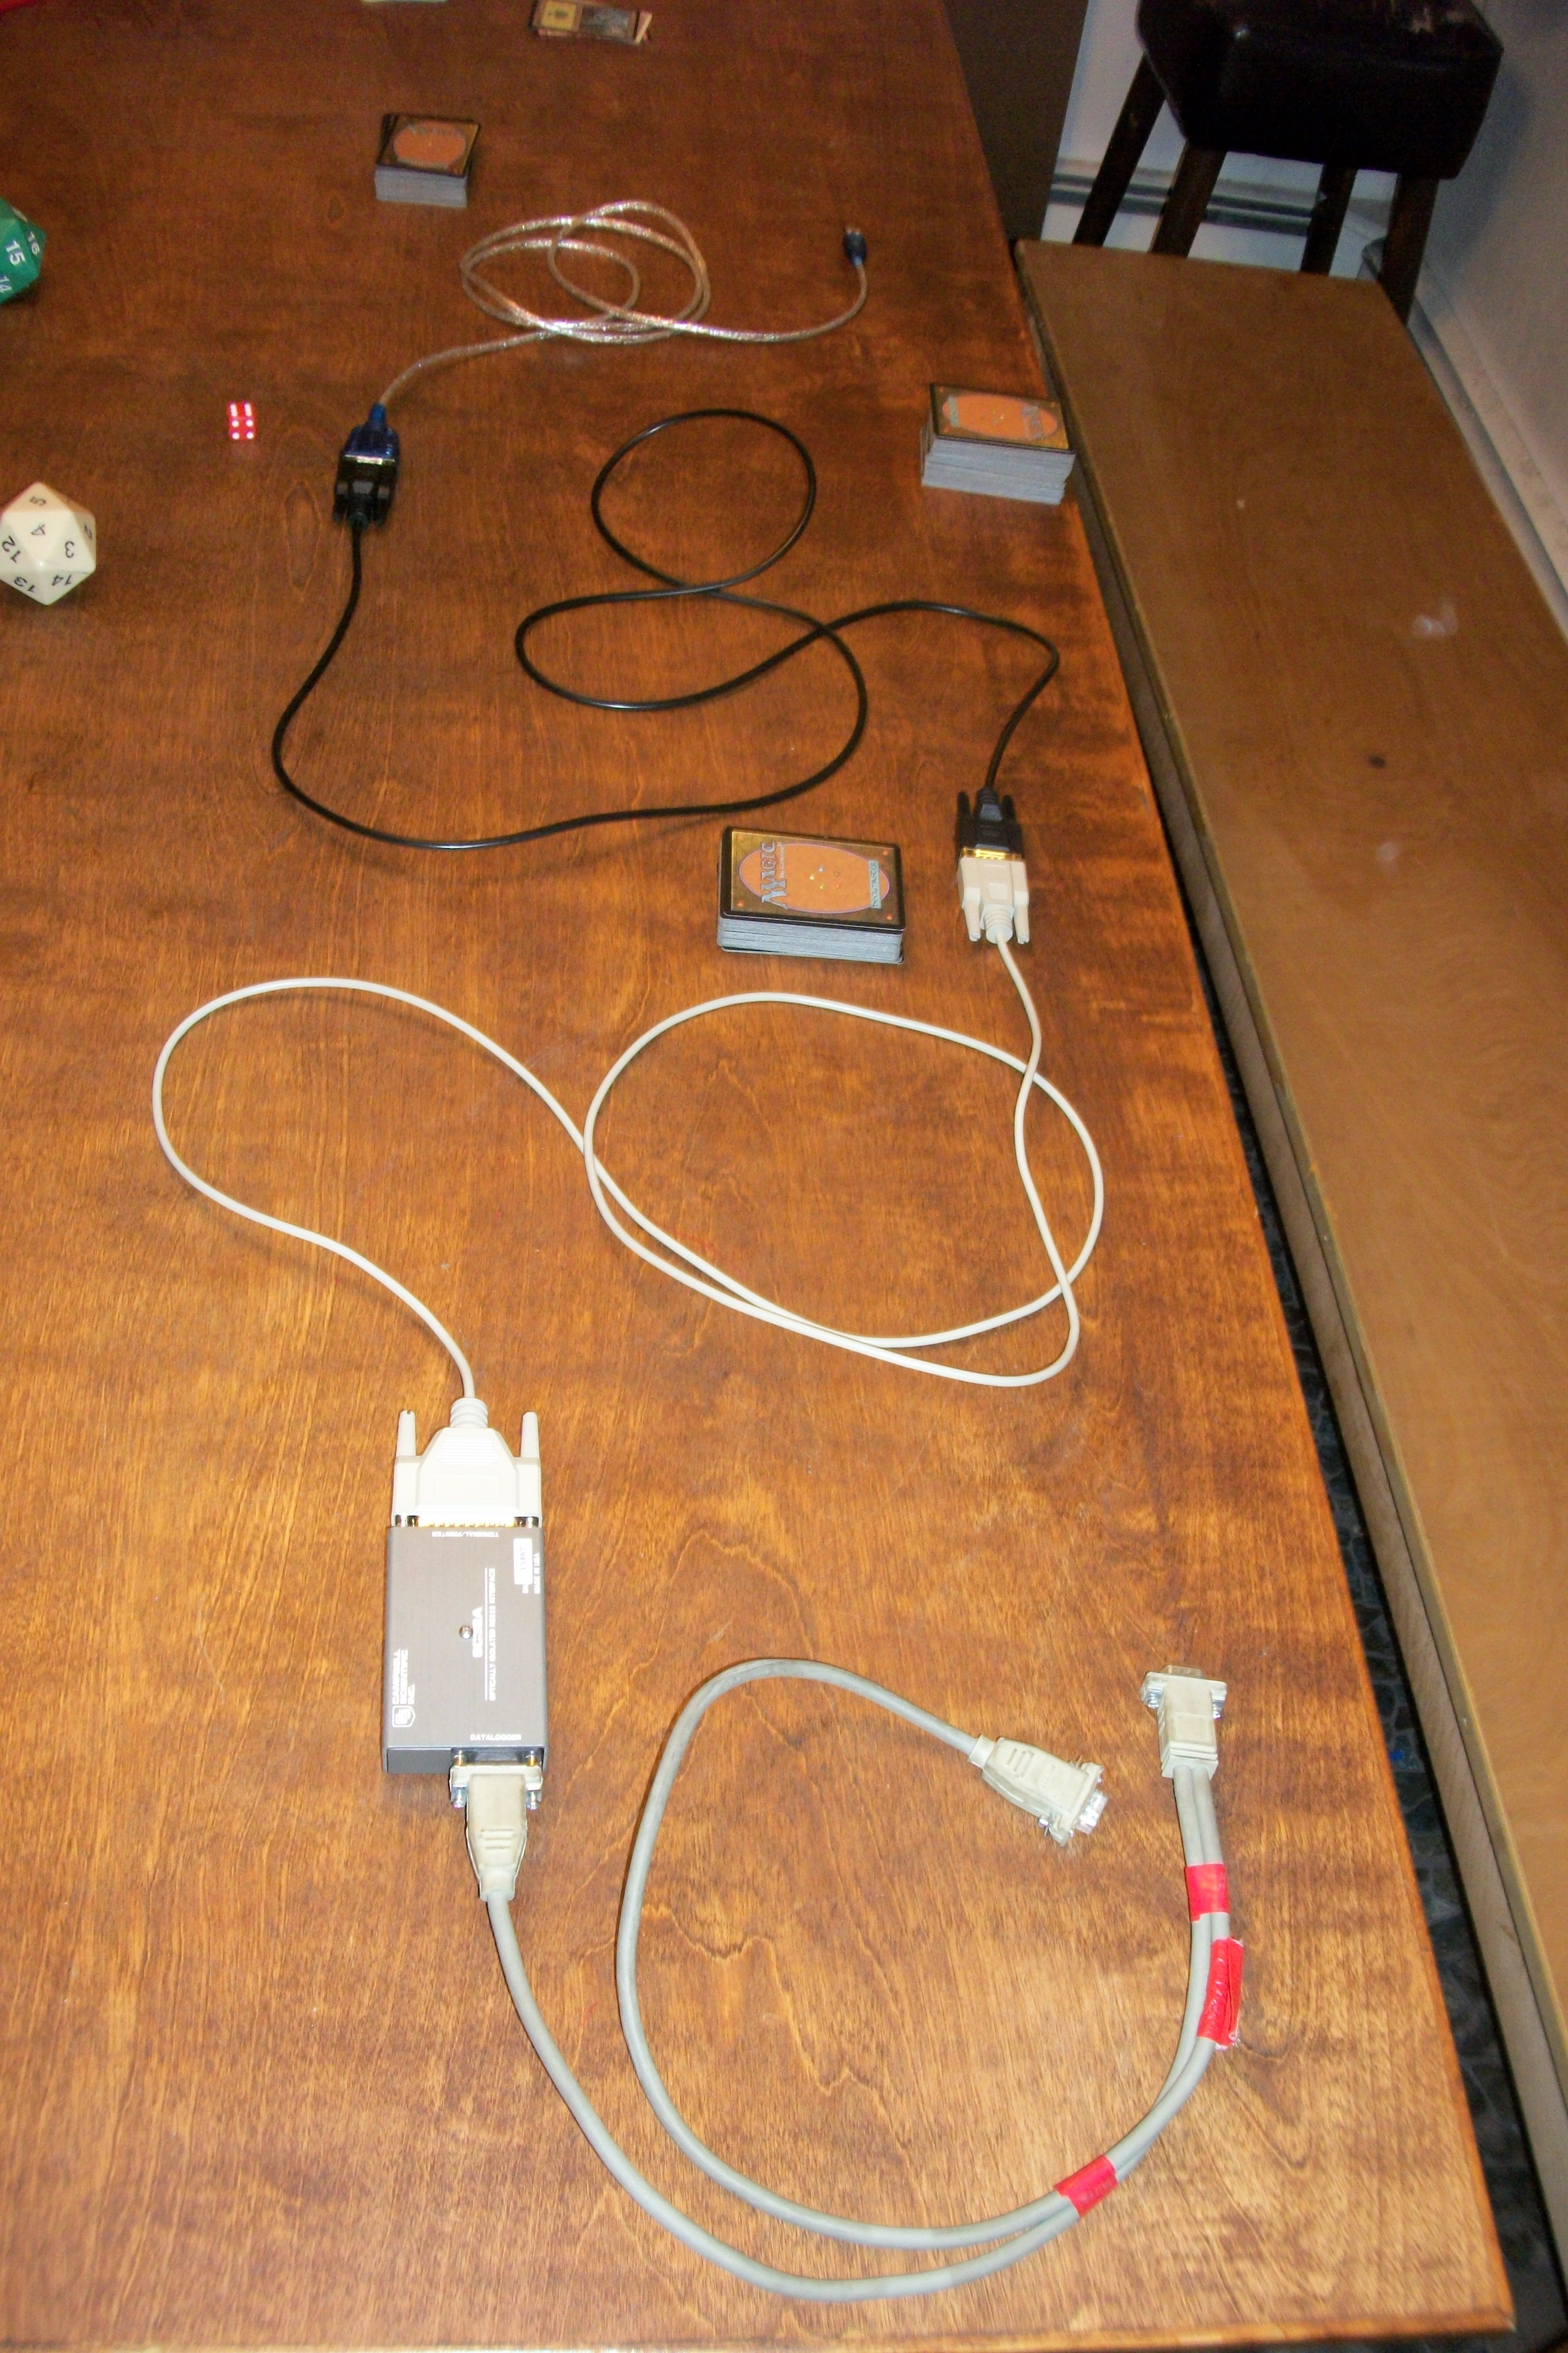
\includegraphics[width=0.6\textwidth]{fig/cable.jpg}
\label{fig:cable}
\caption{The cables used to communicate with the datalogger.}
\end{figure}

Using PC200W, data may be pulled off the CR10X in a raw binary format and then
converted to a CSV format. For this particular experiment, the columns from left
to right represented:

\begin{enumerate}
\item An instrument ID (not used).
\item Ordinal day, out of 366. For example, March 17th is day 76.
\item hh:mm portion of timestamp. For example, 6:30pm is represented as 1830.
\item Seconds portion of timestamp.
\item Needle temperature, in Celcius.
\item Reference temperature, in Celcius.
\item Voltage across needle probe, in millivolts.
\item Experiment timer, in seconds.
\end{enumerate}

This csv data may be analyzed with either spreadsheet software, a series of
scripts, or both. For this series of experiments, Excel and Gnumeric were used
to verify the existence of data and to combine datasets, while python was used
for the analysis.

\marginpar{Organization?}
Generally, each measurement also has some metadata associated with it. In
particular, anisotropic measurements have an angle associated with them, and
snow measurements also have a coordinate position on the snowpack associated
with them. These are measured with a protractor and a tape measure,
respectively. This means that, while taking measurements, one has to be careful
to make sure that they can keep the proper metadata associated with each
measurement. An unfortunate situation that can occur after a long series of
measurements may recall memories of finishing an SAT section and realizing that
you missed a question part-way through. \marginpar{appropriate?}

\begin{figure}[h]
\centering
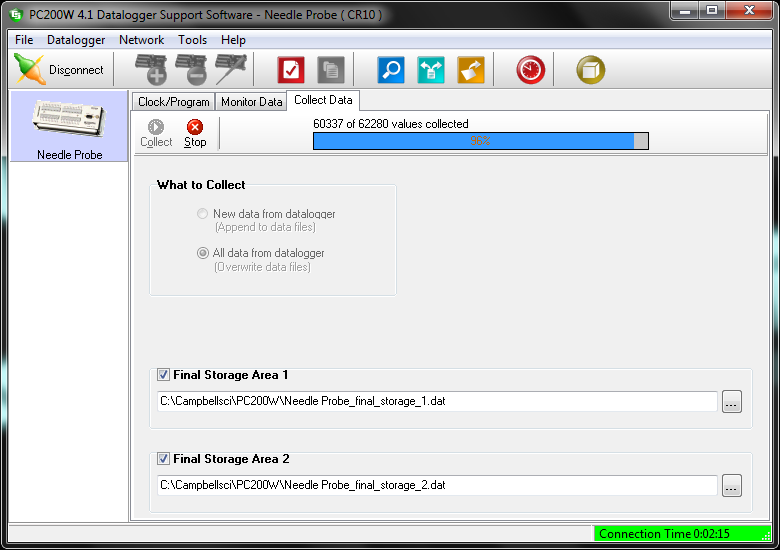
\includegraphics[width=0.8\textwidth]{fig/pc200w.png}
\label{fig:pc200w}
\caption{A screenshot of PC200W, the software used to pull data off the CR10X data logger.}
\end{figure}

Unlike the case of numerical experiments, it is extremely important in
real-world experiments---especially in the case of snow---to hand-inspect every
time/temperature curve. This is because, unlike the numerical experiments, there
is a significant chance that data will be garbage. In the case of snow in
particular, convection is typically experienced near the end of the heating
curve and the beginning of the cooling curve.

\begin{figure}[h]
\centering
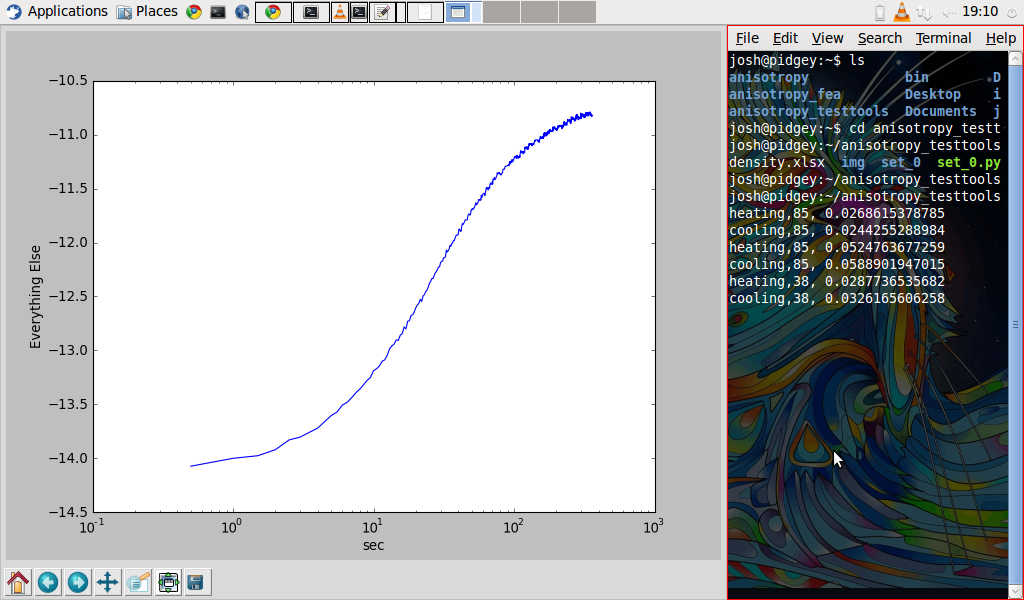
\includegraphics[width=0.8\textwidth]{fig/measurement_graph.png}
\label{fig:meas_graph}
\caption{A plot of time vs. temperature from a real-world measurement of snow.
Each curve must be analyzed by-hand to check for such effects as convection.}
\end{figure}

\section{Snow Conductivity Measurements}

The first step in measuring proper snow was to make a vertical cut in the
snowpack, as in figure \ref{fig:snowpack}.

\begin{figure}[h]
\centering
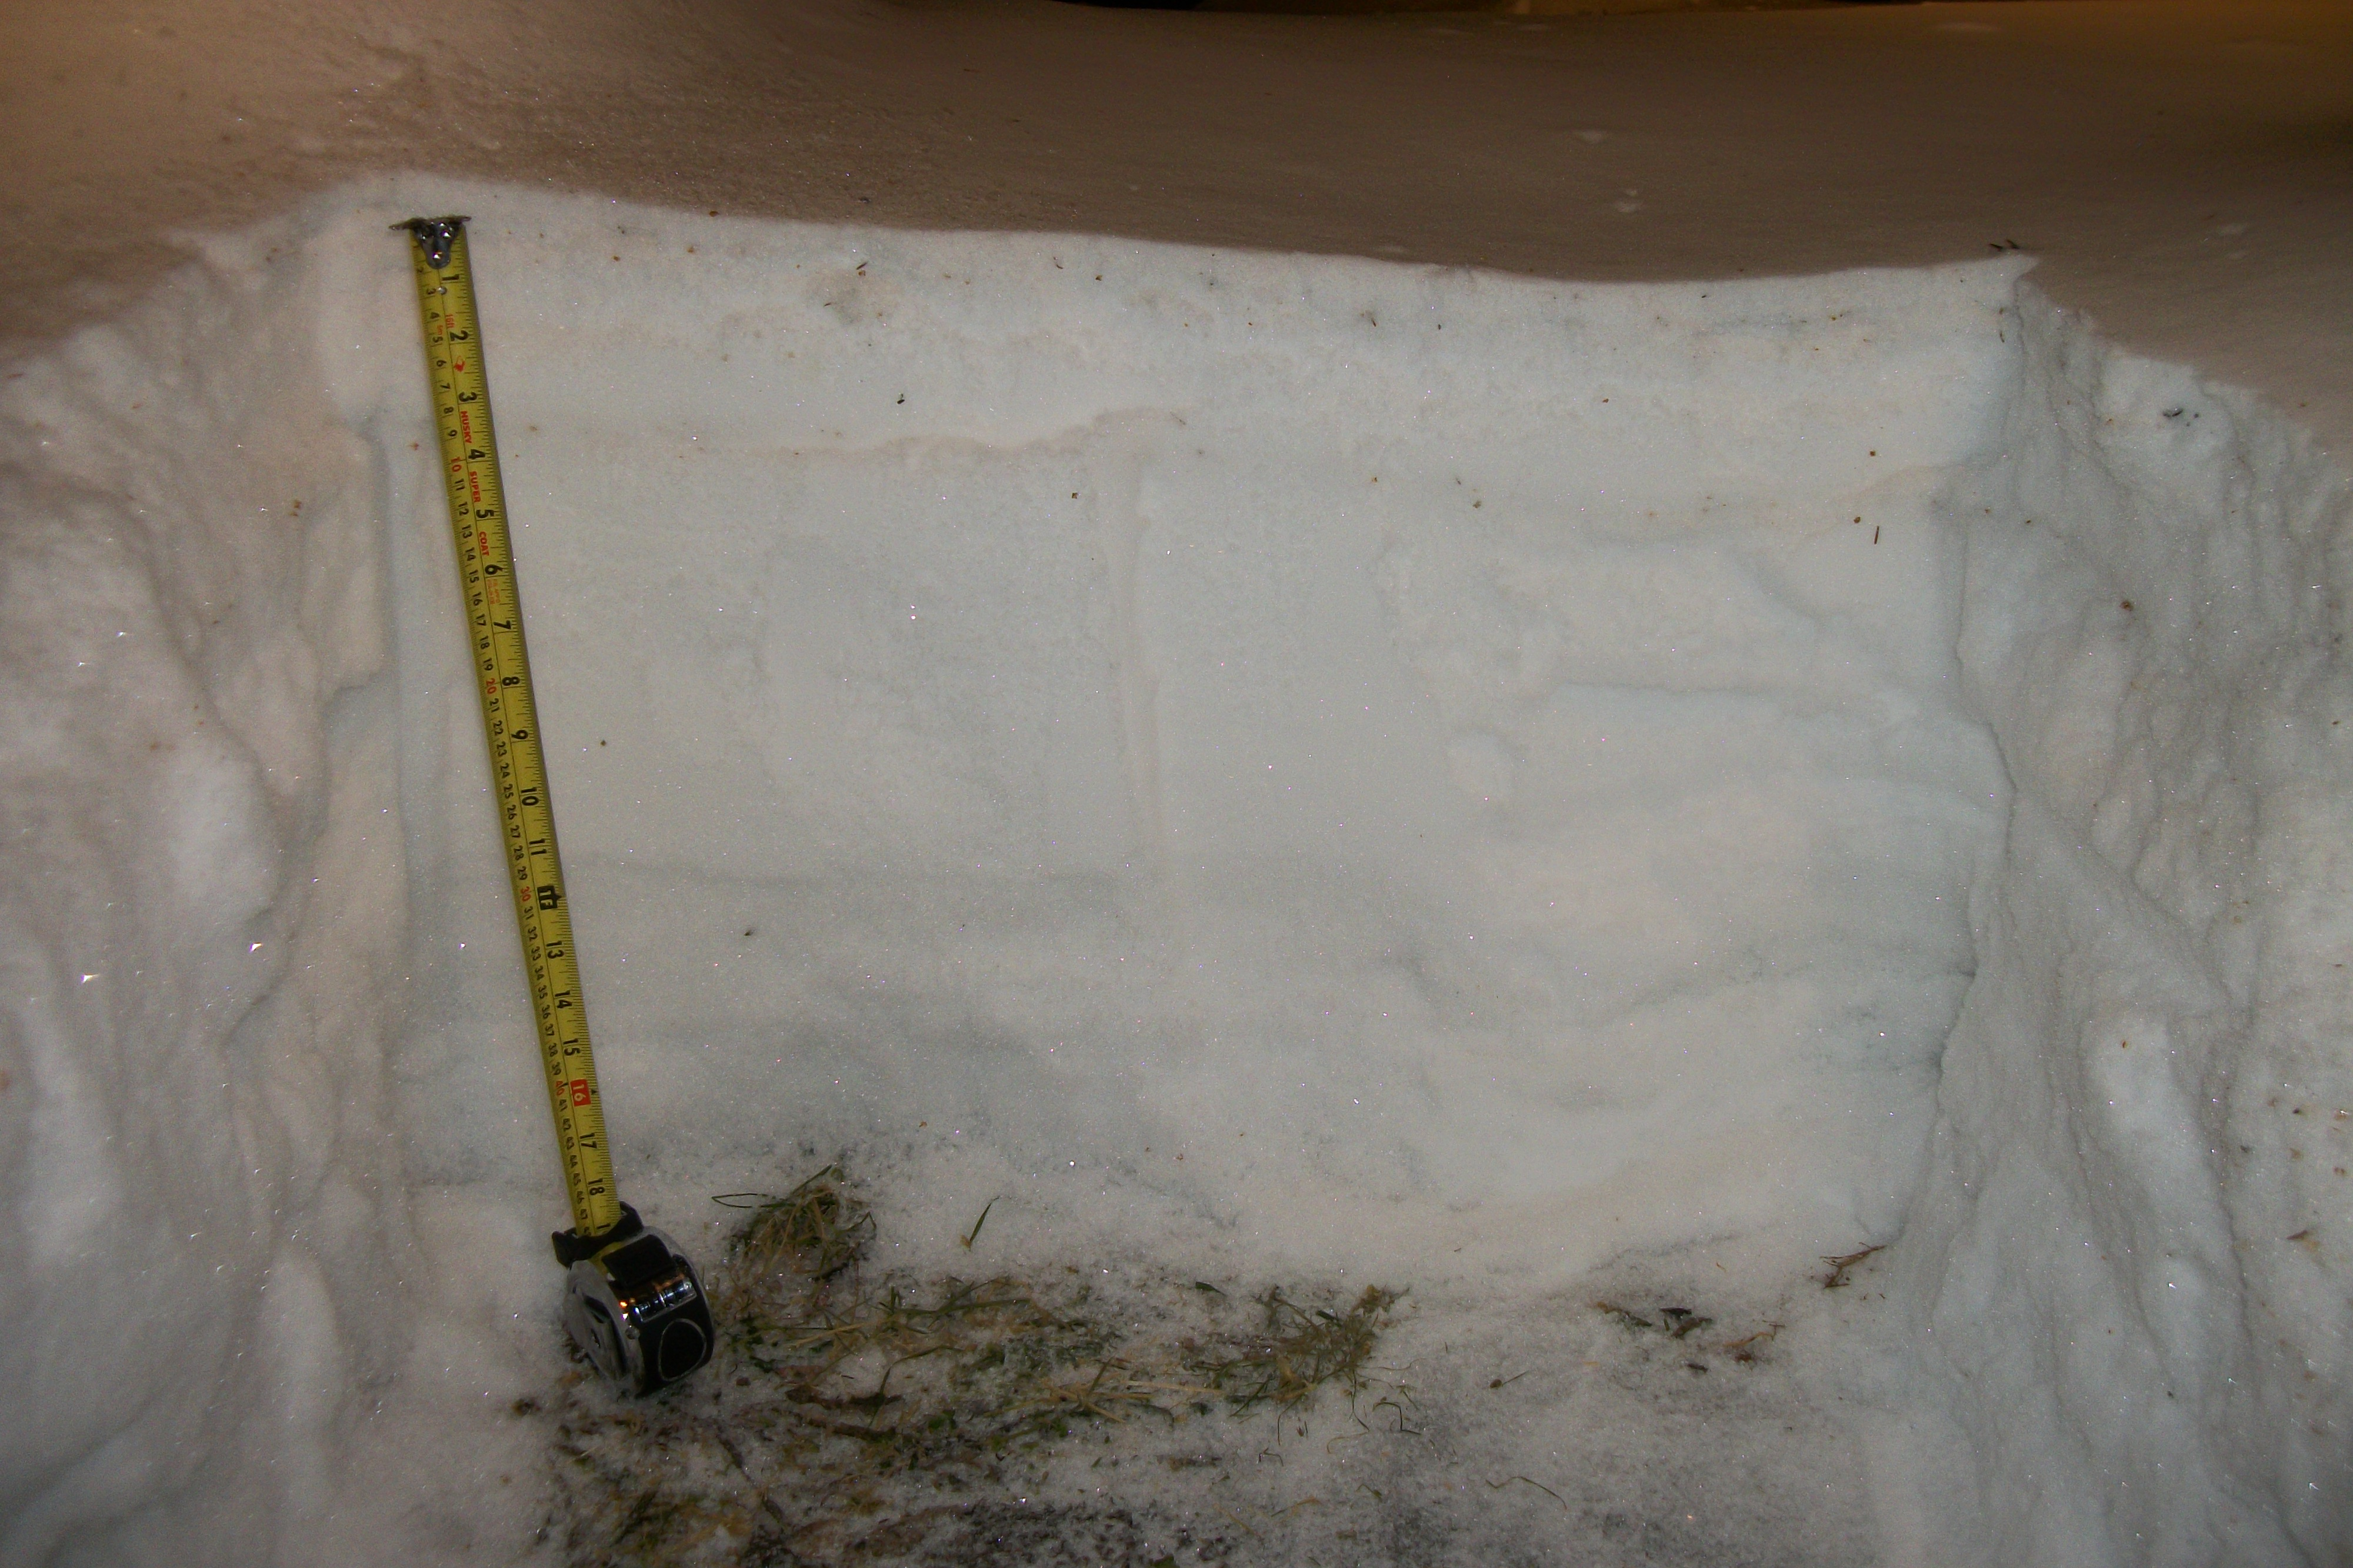
\includegraphics[width=0.8\textwidth]{fig/snowpack.jpg}
\label{fig:snowpack}
\caption{A close-up shot of tested snowpack.}
\end{figure}

Then, for every measurement, the needle was inserted into snow and a measurement
was taken. Snow is relatively difficult to work with due to the low structural 
integrity of the material.  The wire connecting the probe to the data logger is
stiff enough a low temperatures that situating the needle without ruining the
snowpack can be quite a challenge.

Along with each conductivity measurement, the height from the ground---measured
with a tape measure---and the angle of insertion---measured with a protractor
and a plumb bob---were recorded as metadata.

In addition, for each series of measurements at a particular region, the density
of the snow was also measured with cardboard cylinder (used as a control volume)
and a scale.

\begin{figure}[h]
\centering
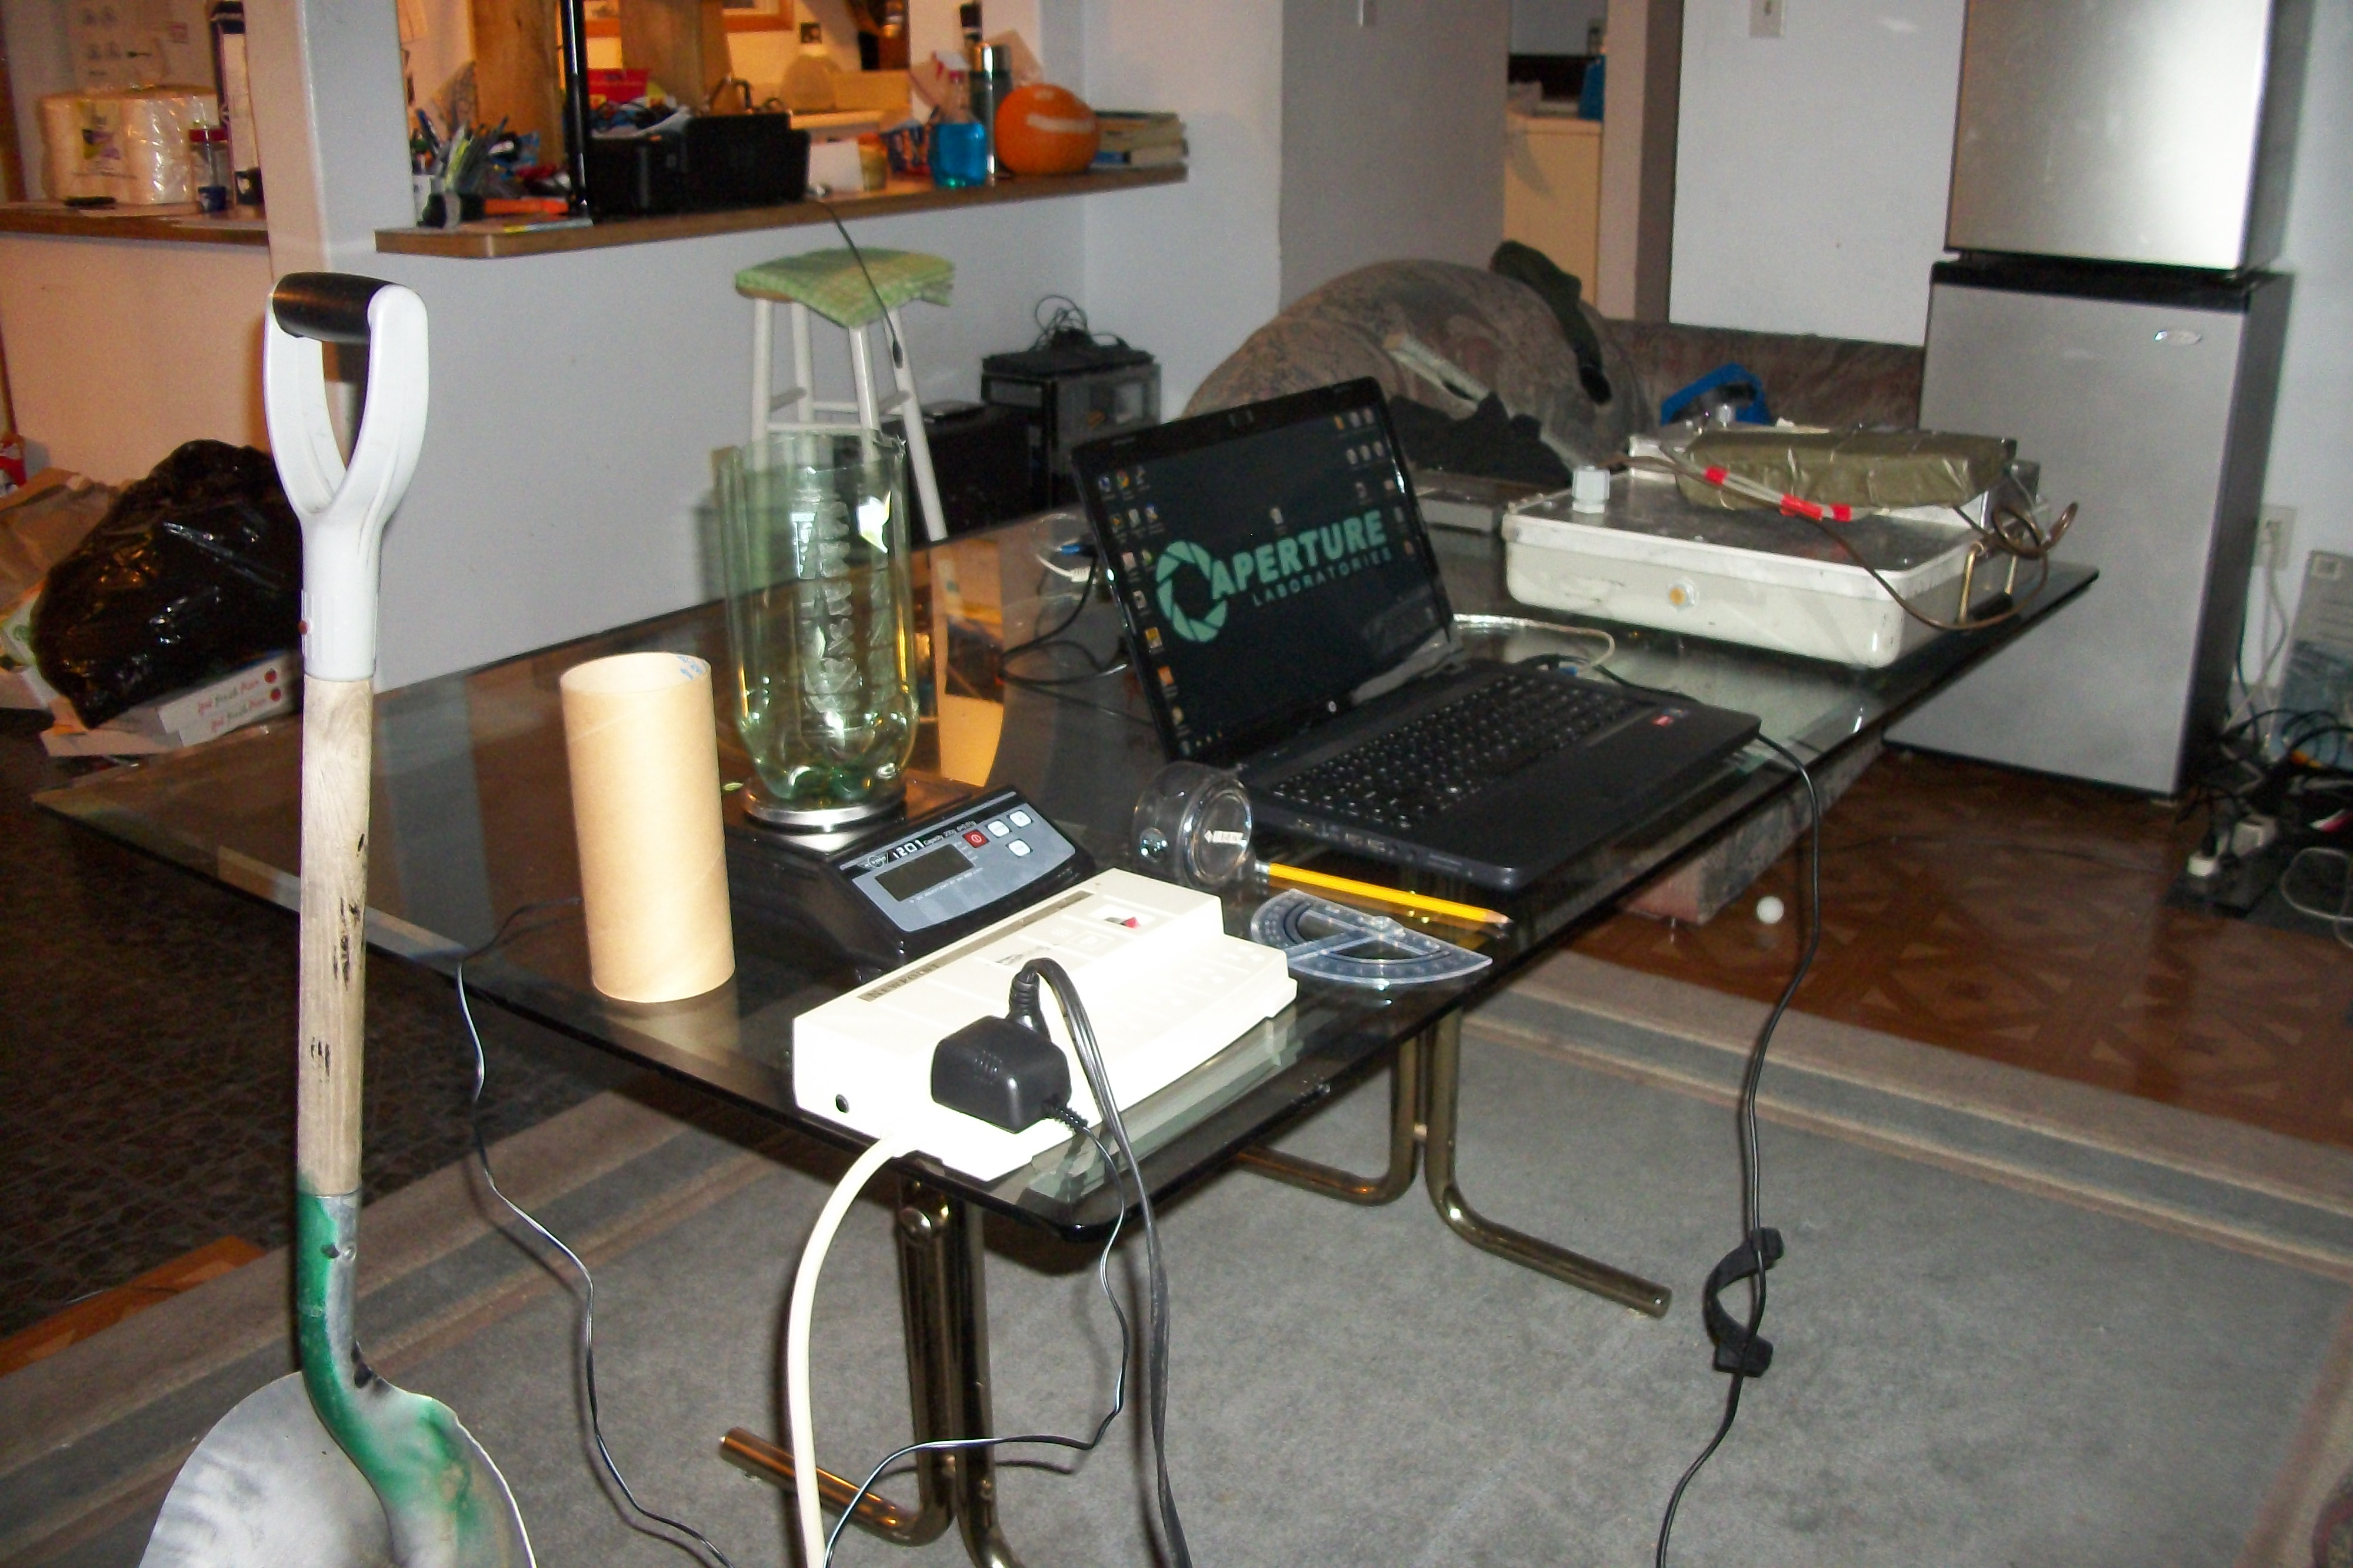
\includegraphics[width=0.8\textwidth]{fig/equipment.jpg}
\label{fig:equipment}
\caption{Equipment used to measure snow thermal conductivity.}
\end{figure}

Data management was problematic, and techniques needed to be developed to handle
it. To ensure that no data was lost, after every measurement data was copied and
appended to the end of a version-controlled csv, and analyzed before the next
measurement was complete. This allowed for mistakes to be caught and undone so
that every measurement could be used. However, metadata management was still
difficult.

\begin{comment}
\begin{figure}[h]
\centering
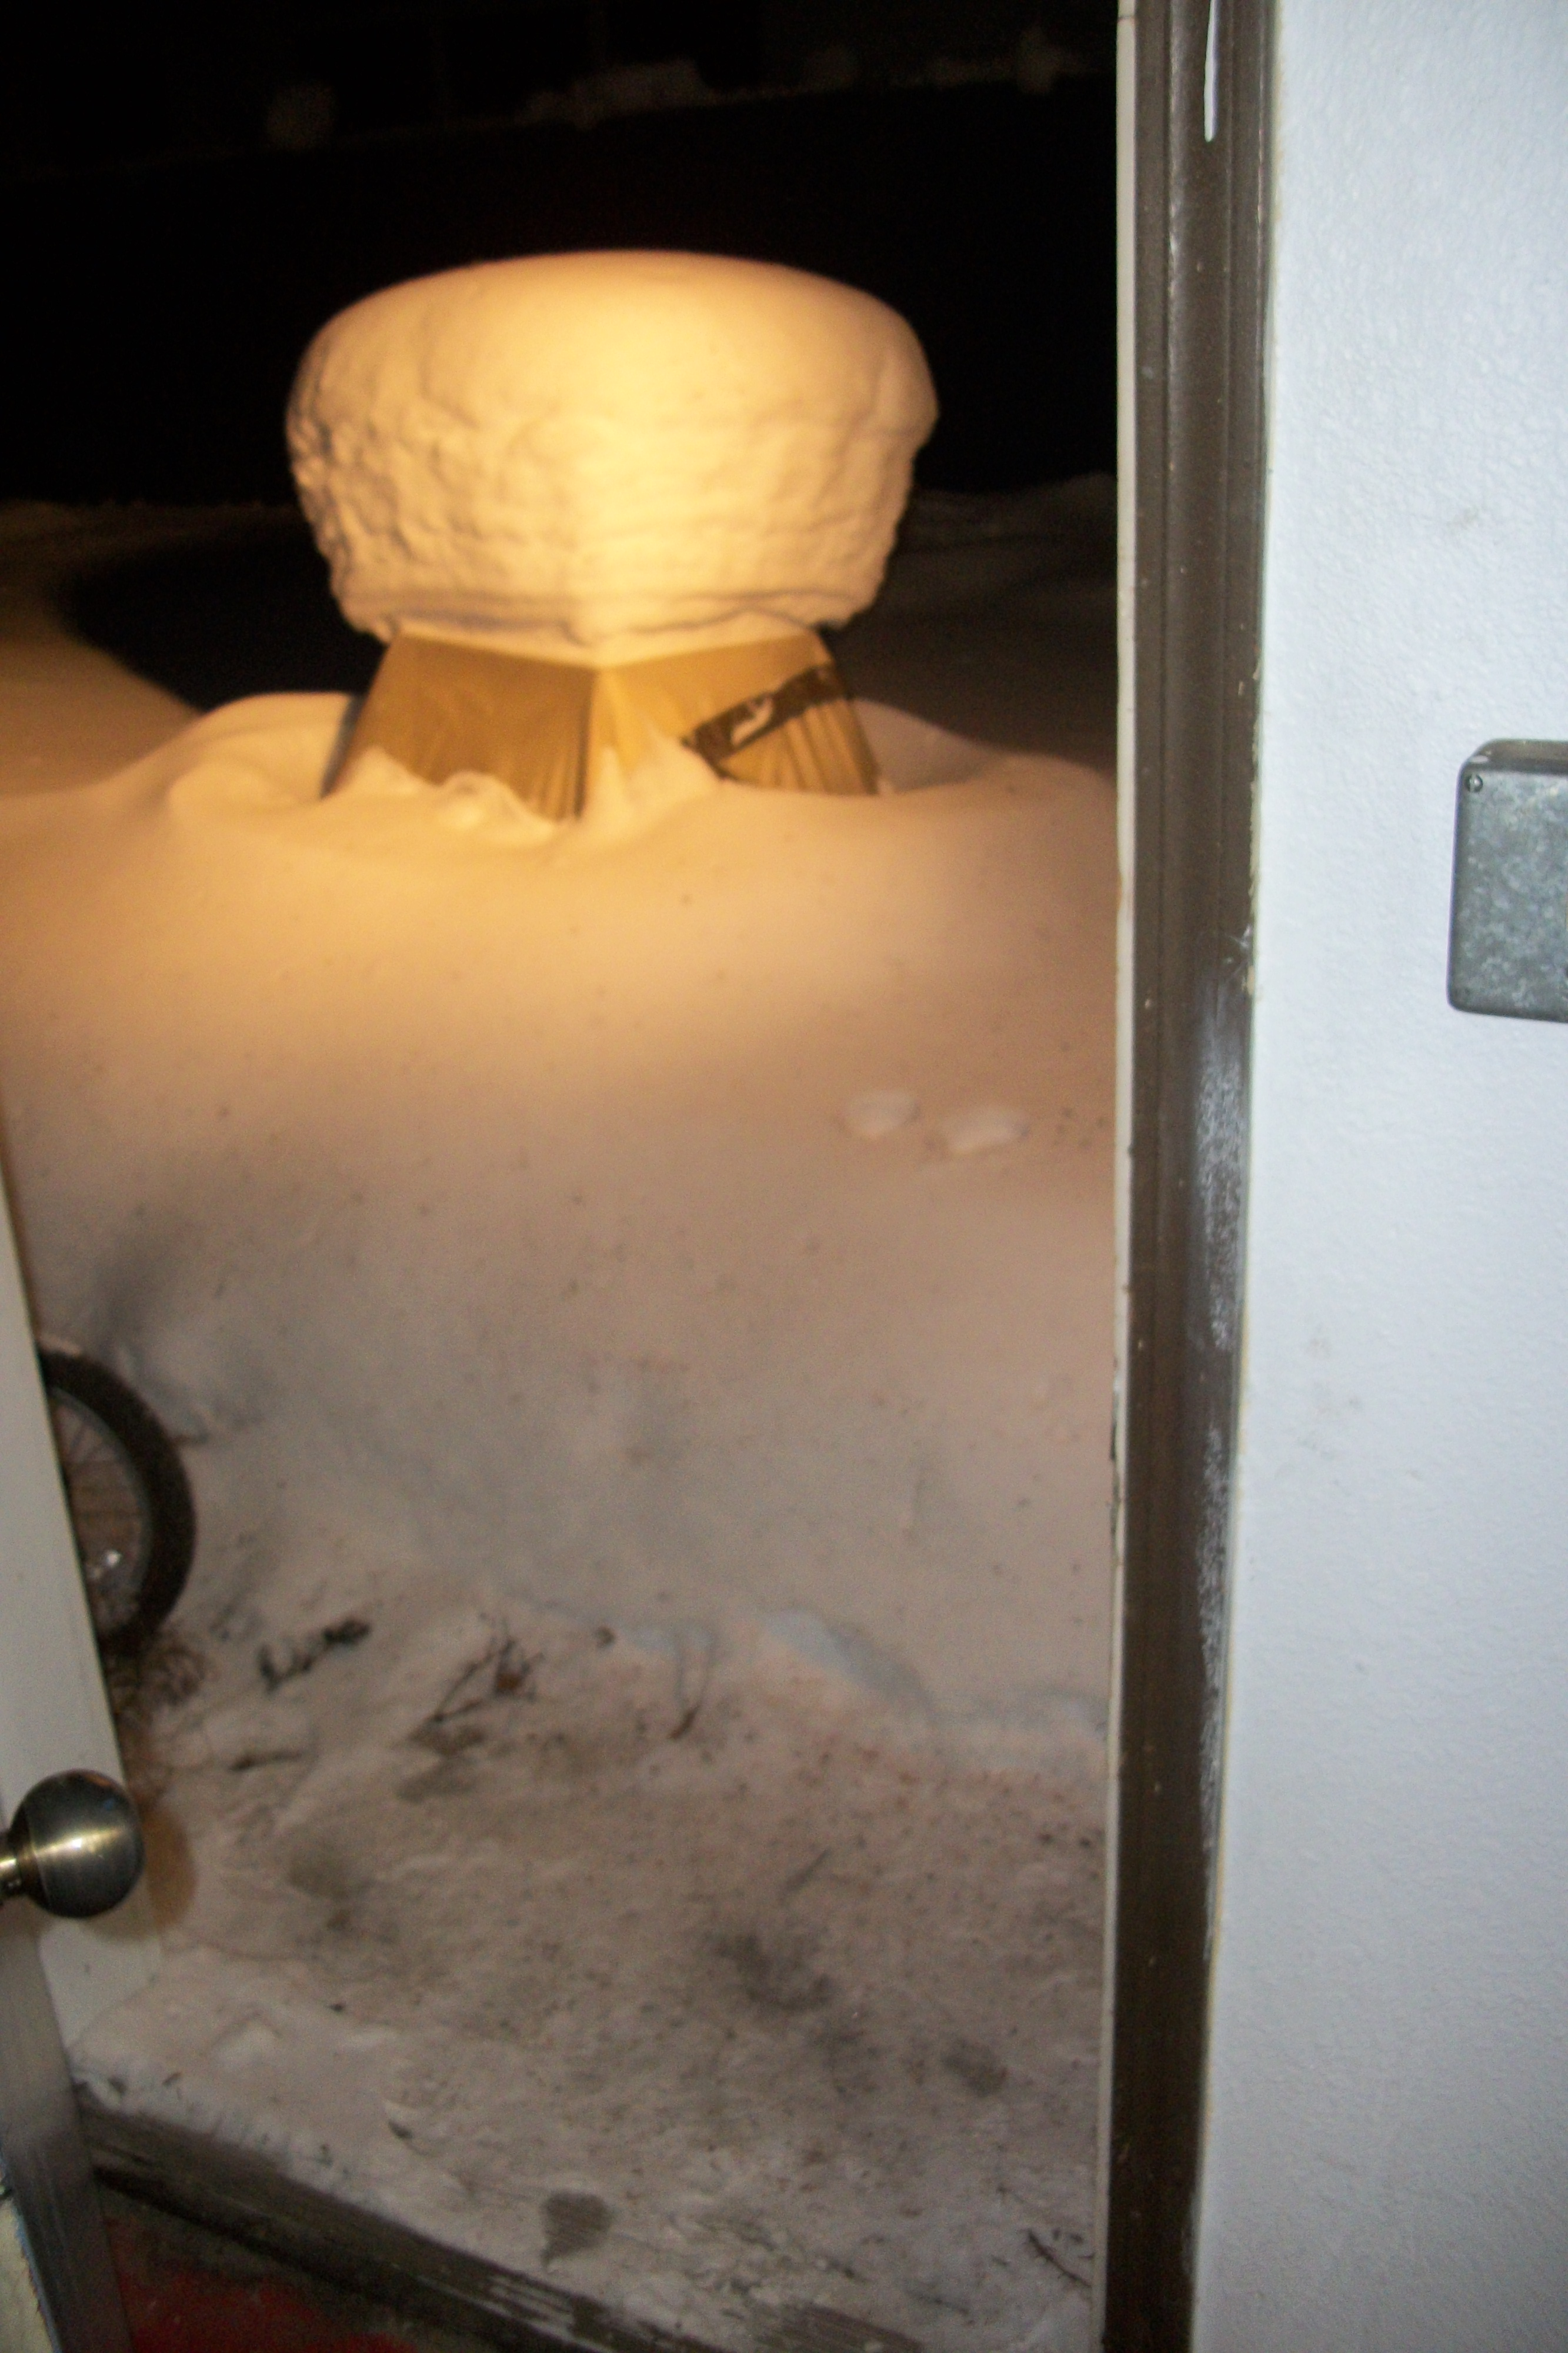
\includegraphics[width=0.4\textwidth]{fig/insitu_location.jpg}
\label{fig:insitu_location}
\caption{The location for in-situ tests.}
\end{figure}
\end{comment}

\section{Benchtop Tests}

A standard used to benchmark needle probes is to measure the conductivity of a
large Nalgene bottle full of glycerine and surrounded in insulating foam to
mitigate changes in room temperature. Glycerine was chosen because, while it
should have the same conductivity of water, does not readily convect. Moreover,
glycerine does not leave an air gap between the needle and the surrounding
medium like many porous materials, such as snow, will. -

A method for testing anisotropic measurements by using alternating alternating
layers of more-conductive and less-conductive materials was devised, based on
this glycerine benchmark test. However, instead of glycerine, the materials
used were table salt and table sugar.

\section{Raw Materials for the Anisotropic Composite}

Salt and sugar's conductivities alone were both measured using the needle probe
apparatus. These measurements resulted in conductivities of
\(0.225\) \(\textrm{W}/\textrm{m}^2/\textrm{K}\) and 
\(0.106\) \(\textrm{W}/\textrm{m}^2/\textrm{K}\), respectively.

\marginpar{Table in appendix!}

Assuming alternating layers of equal thickness, the anisotropic thermal
conductivities in the aggregate should be:

\begin{align}
k_{xy} &= \frac12 \left( k_{\textrm{salt}} + k_{\textrm{sugar}} \right) &= \boxed{0.166}\\
k_z &= 2 \left( \frac1{k_{\textrm{salt}}} + \frac1{k_{\textrm{sugar}}} \right)^{-1} &= \boxed{0.144}\\
\frac{k_z}{k_{xy}} &= \boxed{0.870}
\end{align}

Despite the conductivity of table salt being roughly twice that of sugar, the
anisotropic conductivity ratio is fairly close to 1, meaning that the anisotropy
of the experimental medium, while significant, is relatively weak. On the plus
side, salt and sugar are relatively cheap media to work with.


\section{Apparatus for Containing Anisotropic Composite}

\begin{figure}[h]
\centering
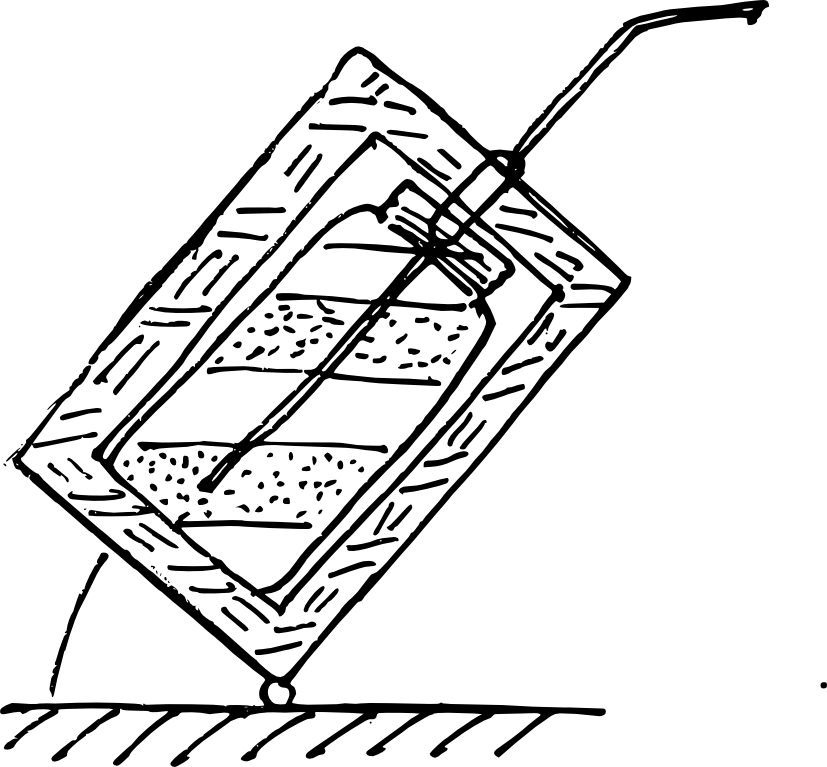
\includegraphics[width=0.4\textwidth]{fig/tilter.png}
\label{fig:tilter}
\caption{An illustration of the tilting apparatus.}
\end{figure}

In order to effectively change the directions of anisotropy, a foam box for the
nalgene bottle was built that could be rotated on an axis and clamped in place.
The resulting angle from the horizontal can be measured with a protractor. The
original plan called for using gels such as glycerine, such that the layers
would self-level. However, because powders were used instead of gels, leveling
had to be done by hand, usually with a spoon. The sugar was dyed green in order
 to differentiate it from the salt.

\section{Measurement Procedure}

Unlike the case of snow, keeping track of measurements was easier for a number
of reasons: First, each measurement was handled at once. Second, each angle
was measured multiple times, and completely finished before other angles were
measured. Each angle measured was measured at least three times, and up to five
or more if clean measurements proved elusive.

\section{Conclusion}

ihnfi
